\subsection{Improved K-Means}
\label{subsec:improvedkmeansresults}

This section provides an overview of the results obtained from the improved K-Means algorithms implemented, Global K-Means and G-Means.

\subsubsection{Global K-Means}
\label{subsec:globalkmeansresults}

We found that the number of clusters has a significant impact on the F-measure,
as shown in Figure \ref{fig:interactions-global-kmeans}. For both the Mushroom and Hepatitis datasets, the F1 score was
highest with a lower number of clusters, and steadily decreased as the number of clusters increased. For the Vowel dataset, the F1 score was lowest 
with a small number of clusters, and increased as the number of clusters increased. These results are consistent with the number of classes in each
dataset— 2 for Mushroom and Hepatitis, and 11 for Vowel.

\begin{figure}[h!]
    \centering
    \includegraphics[width=0.5\textwidth]{figures/interactions_global_kmeans.png}
    \caption{Interactions between hyperparameters in Global K-Means}
    \label{fig:interactions-global-kmeans}
\end{figure}

Adjusting the tolerance parameter had a negligable impact on the F-measure, as shown by the plots appearing to have the same colour across
all 3 datasets. One possible explanation for this is in Global K-Means, the tolerance parameter only influences the convergence criteria
of the K-Means subroutine used at each step of the algorithm. As long as K-Means converges successfully for a given number of clusters, the
overall clustering results are unlikely to be affected. This suggests that the initial placement of the centroids and
the maximum number of clusters are more important than the tolerance parameter in Global K-Means.


\subsubsection{G-Means}
\label{subsec:gmeansresults}

Compared to Global K-Means, the results are more varied for G-Means as shown in Figure \ref{fig:interactions_gmeans}.
The strictness parameter affects the F-measure differently across datasets. For the Mushroom dataset, strictness has
negligible impact on the F-measure but produces outlier scores at every level. For the Vowel dataset, strictness similarly
has negligible impact, with no outliers observed. In contrast, the Hepatitis dataset shows the most variation in F-measure,
with wider distributions and multiple outliers, indicating greater sensitivity to the strictness parameter.



\begin{figure}[h!]
    \centering
    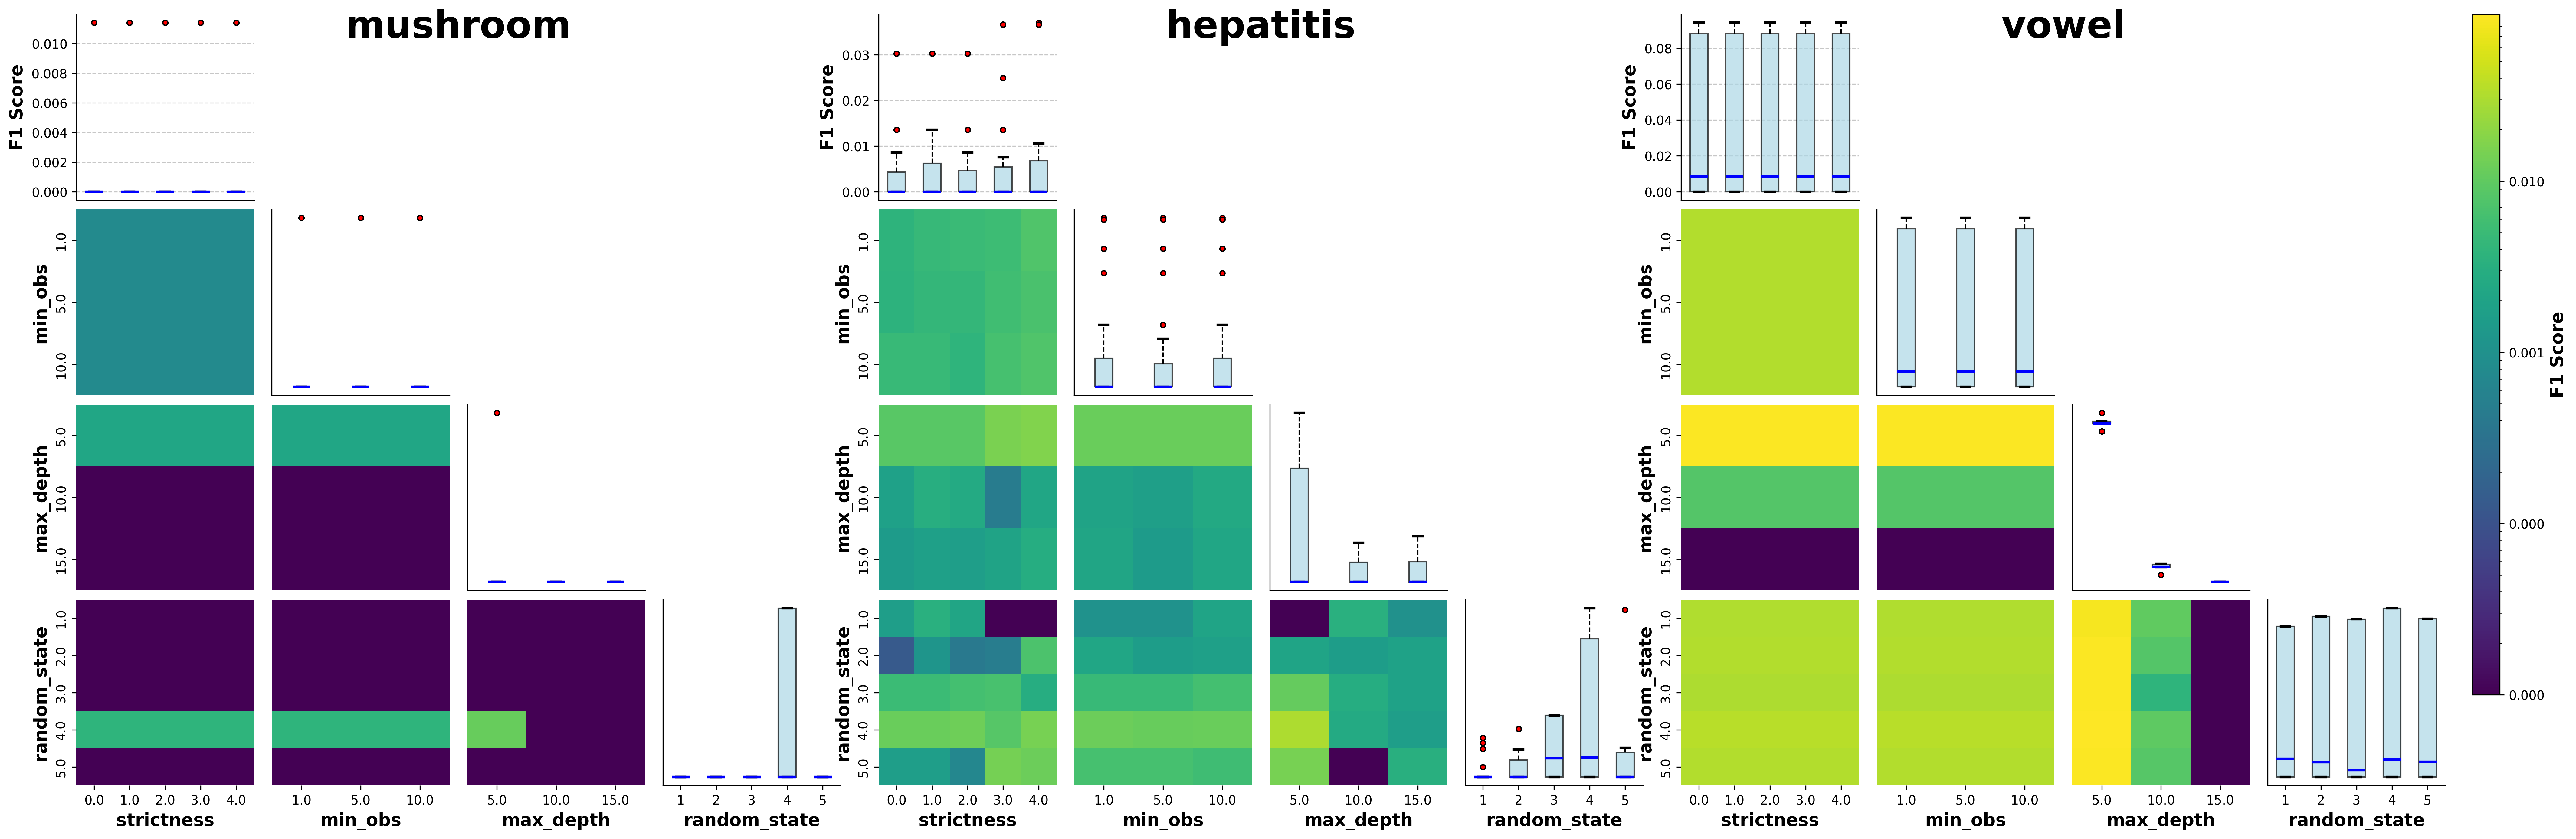
\includegraphics[width=0.5\textwidth]{figures/interactions_gmeans.png}
    \caption{Interactions between hyperparameters in G-Means}
    \label{fig:interactions_gmeans}
\end{figure}



